\section{Durchführung}
\label{sec:Durchführung}

\begin{figure}
    \centering
    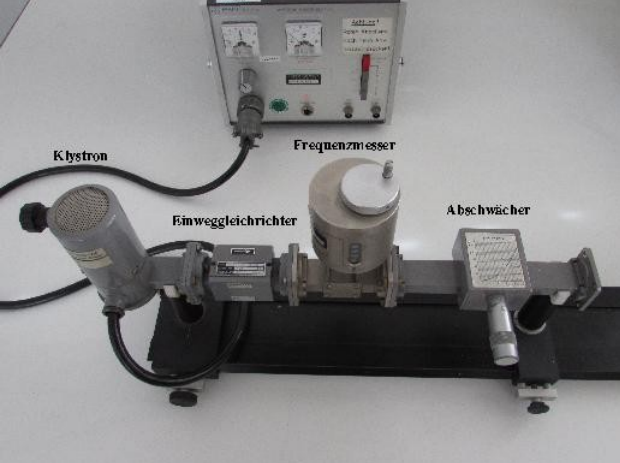
\includegraphics[width=0.8\textwidth]{Bilder/grundaufbau.png}
    \caption{Grundlegender Aufbau des Versuchs.}
    \label{fig:grund}
\end{figure}
\FloatBarrier

Der grundlegende Aufbau ist in Abbildung \ref{fig:grund} zu sehen. Der Teil, mit dem die Mikrowellen für die weitere Vermessung erzeugt wird, bleibt über den 
gesamten Versuch gleich. Das Reflexklystron, dessen Spannung variabel ist, emittiert Mikrowellen, die per Hohlleiter über den gesamten Aufbau weitergeleitet werden. Als 
erstes treffen diese auf einen Einweggleichrichter, der Rückflussresonanzen unterdrückt und somit Messfehler durch Störungen bei Erzeugung der Mikrowellen vorbeugt. Es folgt ein Frequenzmesser und darauf eine Dämpfungseinheit,
die die Intensität der Mikrowellen abschwächt. Für die weiteren Teilversuche werden nach Bedarf die weiteren Komponenten hinzugefügt.

\subsection{Untersuchen der Moden}

Hierfür wird die Dämpfung auf $\SI{30}{\decibel} $ gestellt und am Klystron der $\SI{50}{\mega\hertz} $-Modus verwendet.
Der Aufbau wird hierfür um eine Diode erweitert. Des Weiteren bildet ein Oszilloskop, welches im xy-Modus (x: Reflektorspannung , y: Messstelle Hohlleiter) 
betrieben wird, die Modenverläufe ab. Mit dem Frequenzmesser kann eine Frequenz, die im Frequenzband einer Mode liegt, getroffen werden, wodurch es an dieser Stelle zu einem 
Leistungseinbruch, der im Folgenden auch als Dip referenziert wird, kommt. Dieser kann dann über die Höhenverstellung am Klystron so verschoben werden, dass der Dip genau am 
Maximun der Mode liegt. Außerdem wird der Dip noch jeweils auf beiden Seiten auf die halbe Höhe der Amplitude verschoben. Damit können die Amplitudenverhälnisse, und die jeweiligen 
Frequenzen abgelesen werden. Dieser Vorgang wird für drei verschiedene Moden wiederholt. In der Abbildung \ref{fig:dip} die Messpunkte an den Moden schematisch dargestellt. 

\begin{figure}
    \centering
    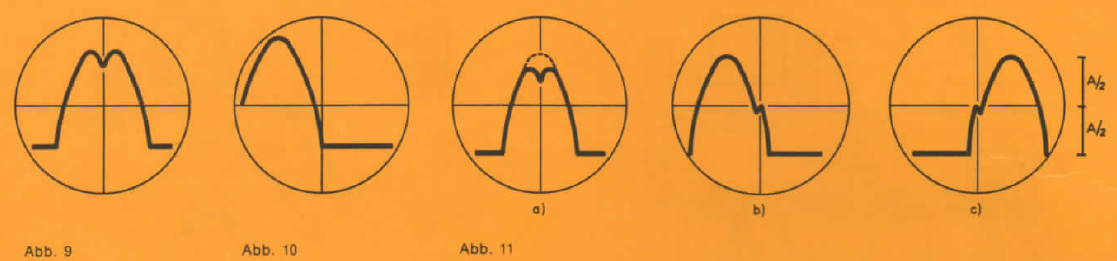
\includegraphics[width=0.8\textwidth]{Bilder/dip.png}
    \caption{Schematische Darstellung der zu vermessenen Punkte.}
    \label{fig:dip}
\end{figure}
\FloatBarrier

\subsection{Hohlleiterfrequenz}

\begin{figure}
    \centering
    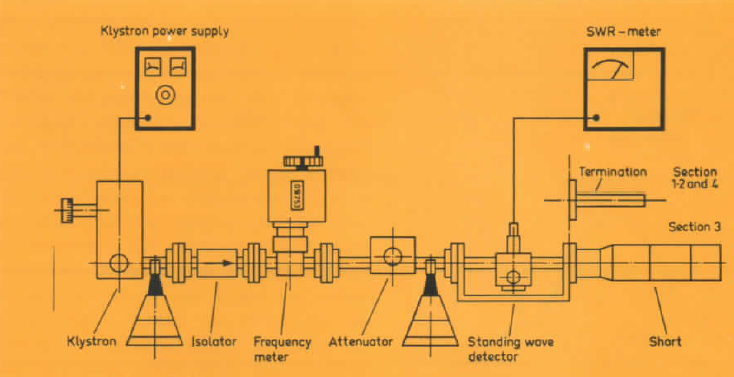
\includegraphics[width=0.8\textwidth]{Bilder/aufbau_freq.png}
    \caption{Versuchsaufbau für Messung von Frequenz, Dämpfung und Wellenlänge.}
    \label{fig:hohl}
\end{figure}
\FloatBarrier

Es wird hier der $\SI{1}{\kilo\hertz} $-Modus mit einer Dämpfung von $\SI{20}{\decibel} $ verwendet und der Versuch wie in der Abbildung \ref{fig:hohl} erweitert. Mit dem Frequenzmesser wird 
nach der Frequenz gesucht, bei der ein minimaler Ausschlag am SWR-Meter gemessen wird, und diese notiert. Daraufhin wird der Abschluss am Ende des Hohlleiters wieder durch einen 
Kurzschluss ersetzt. Nun wird die Messsonde verschoben, bis wieder ein Minimum am SWR-Meter zu sehen ist und die Position der Messonde notiert. Danach wird diese weiter bis zum 
nächsten Minimum verschoben und die Position notiert. 

\subsection{Dämpfung}
Für die Untersuchung der Dämpfung wird wieder ein Abschluss anstelle des Kurzschlusses montiert. Das SWR-Meter wird vorab kalibriert und die Dämpfung wird variiert. Dabei werden 
in $\SI{2}{\decibel} $ Schritten die eingestellte Dämpfung notiert. 

\subsection{Welligkeitsverhältnis}

Die Bestimmung des Welligkeitsverhältnisses geschiet über drei verschiedene Methoden. Der Aufbau bleibt dabei für alle Methoden der Gleiche. Dieser ist in der Abbildung \ref{fig:swr} zu sehen.

\begin{figure}
    \centering
    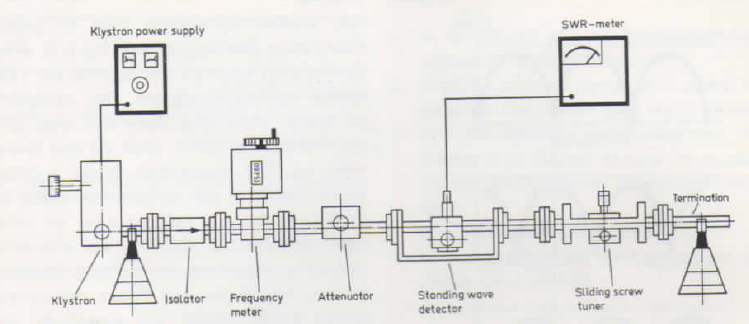
\includegraphics[width=0.8\textwidth]{Bilder/aufbau_swr.png}
    \caption{Versuchsaufbau zur Messung des Stehwellenverhältnisses.}
    \label{fig:swr}
\end{figure}
\FloatBarrier


\subsubsection{Direkte Methode}
 
Bei einer konstanten Stifttiefe wird die Messsonde bis zu einem Maximun verschoben, wonach das SWR-Meter auf 1 normiert wird, indem die Verstärkung des SWR-Meters variiert wird. Danach wird sie zu
einem Minimum verschoben um das Stehwellenverhältnis ablesen zu können. Dies wird für die Stifttiefen 3,5,7 und 9 $\si{\mm}$ durchgeführt.

\subsubsection{3 dB Methode}
Bei einer Stifttiefe von 9 mm wird die Sonde in ein Minimum verschoben und das SWR-Meter auf 3 dB eingestellt. Daraufhin wird die Sonde verschoben, bis 
der Ausschlag auf dem SWR-Meter 0 dB anzeigt und die Sondenposition notiert. Das gleiche Verfahren wird in die andere Richtung des Minimums durchgeführt, bis auch wieder 0 dB 
abzulesen sind. Danach wird der Abschluss durch einen Kurzschluss ersetzt und der Abstand der Sonde zwischen zwei Minima abgelesen.


\subsubsection{Abschwächermethode}
Die Stifttiefe ist hierfür wieder auf 9 mm eingestellt und die Sonde wird wieder zu einem Minimum verschoben. Die Dämpfungseinheit wird auf 20 dB eingestellt und das SWR-Meter im 
Minimum auf 3 dB angepasst. Daraufhin wird simultan die Sonde in Richtung eines Maximums verschoben, wobei die Dämpfungseinheit so variiert wird, dass der Ausschlag auf dem SWR-Meter 
bei 3 dB bleibt. Bei Erreichen des Maximums wird dann die eingestellte Dämpfung abgelesen. 
